% =====================================================================
% Cross-Lingual Memory in LLM Agents (course project paper, midsem)
% Template: course ACL template, LuaLaTeX variant (needed for Devanagari).
% COMPILE WITH LuaLaTeX  (Overleaf: Menu > Compiler > LuaLaTeX).
% =====================================================================
\documentclass[11pt]{article}

% "final" shows author names. Use "review" for an anonymous version.
\usepackage[final]{acl}
\usepackage{microtype}

% Fonts (LuaLaTeX). Shobhika is a Devanagari font shipped inside TeX Live, so it is
% always available on Overleaf. HarfBuzz shapes Devanagari conjuncts correctly.
\usepackage[english,bidi=default]{babel}
\babelfont{rm}{TeXGyreTermesX}
\babelprovide[import, onchar=ids fonts]{hindi}
\babelfont[hindi]{rm}[Renderer=HarfBuzz, Extension=.otf, UprightFont=*-Regular, BoldFont=*-Bold]{Shobhika}
\newcommand{\hi}[1]{\foreignlanguage{hindi}{#1}}

\usepackage{graphicx}
\usepackage{booktabs}
\usepackage{multirow}
\usepackage{tabularx}
\usepackage{amsmath}
\usepackage{amssymb}
\usepackage{xcolor}
\usepackage{enumitem}

\newcommand{\TODO}[1]{\textcolor{red}{\textbf{[TODO: #1]}}}
\newcommand{\yes}{$\checkmark$}
\newcommand{\no}{$\times$}
\newcommand{\partly}{$\circ$}
\newcommand{\EN}{\textsc{en}}
\newcommand{\HI}{\textsc{hi}}
\newcommand{\HG}{\textsc{hg}}

\title{Same Memory, Different Language: A Controlled Pilot Study of\\
Cross-Lingual Memory in LLM Agents for English, Hindi and Hinglish}

\author{\TODO{Author 1} \\ \TODO{Institute} \\ \texttt{\TODO{email}} \And
        \TODO{Author 2} \\ \TODO{Institute} \\ \texttt{\TODO{email}} \And
        \TODO{Author 3} \\ \TODO{Institute} \\ \texttt{\TODO{email}}}

\begin{document}
\maketitle

% ---------------------------------------------------------------------
\begin{abstract}
Large language model (LLM) assistants now keep long-term memories of what users tell them, so that later conversations can be personalised.
Existing memory benchmarks are written in English, and they assume that a user stores a fact and later asks about it in the same language.
Multilingual users often switch languages between conversations, and no existing evaluation isolates the effect of this switch.
We therefore present a controlled evaluation in which each personal memory stays fixed while the language used to store it and the language used to ask about it vary independently across English, Hindi and Hinglish.
We compare a model that reads the full conversation history with a retrieval-based memory that stores the original text, an English translation, or both, and we add an oracle condition that separates retrieval errors from reading errors.
In a pilot with 30 memories and two open 8-billion-parameter models, storing an English copy of each memory raised the rate at which keyword search ranked the correct memory first from 29\% to 72\% when the two languages differed.
The language of the question also affected accuracy more than the language of storage.
These findings suggest that memory systems for multilingual users should keep an English representation next to the original text.
\end{abstract}

% ---------------------------------------------------------------------
\section{Introduction}
\label{sec:intro}

LLM-based assistants and agents increasingly persist across sessions.
They store facts, preferences and events that a user discloses, and they retrieve these memories in later conversations.
Systems such as MemGPT~\citep{packer2023memgpt}, MemoryBank~\citep{zhong2024memorybank}, Mem0~\citep{chhikara2025mem0} and A-MEM~\citep{xu2025amem} manage such external memory stores.
This persistence lets an assistant remember a user's diet, the name of a family member or the date of an upcoming exam.

Many users, however, do not speak to an assistant in a single language.
In India, users write Hindi in its native Devanagari script, write English, and write Hinglish, which is Hindi typed in Roman letters and mixed with English words.
Linguists call such mixing of two languages within one conversation \emph{code-switching}.
A user may tell an assistant \hi{मेरी बिल्ली का नाम लूना है} (``my cat's name is Luna'') in Hindi and ask a month later, in English, ``What's my cat called?''.
If the assistant cannot connect the two languages, it claims ignorance, recalls the wrong fact or invents one.

Current memory benchmarks such as LoCoMo~\citep{maharana2024locomo}, LongMemEval~\citep{wu2025longmemeval} and MemoryAgentBench~\citep{hu2026memoryagentbench} measure whether an agent retains information over long interactions, but all of them are in English.
Work on cross-lingual question answering asks questions about documents written in another language~\citep{lewis2020mlqa,hengle2025mlneedle}, yet it studies encyclopedic text, and it often fixes the question to English.
A recent bilingual memory dataset mixes English and Vietnamese, but each of its questions appears in one language only~\citep{nguyendang2026lhmemory}.
None of this work can tell whether an error comes from the language switch or from the difficulty of a particular question.

We address this gap with a matched design.
Every memory exists in three parallel versions, in English (\EN), Hindi in Devanagari (\HI) and Hinglish (\HG).
We place the memory in a conversation history written entirely in one \emph{storage} language and ask about it in one \emph{query} language.
Crossing the three storage languages with the three query languages gives nine conditions.
Only the language changes between conditions, so a difference in accuracy reflects the language switch.

Our method has four stages, shown in Figure~\ref{fig:method}.
The first stage builds memory items from LongMemEval and writes each one in all three languages.
The second stage embeds each memory in a ten-session history in the storage language, together with unrelated filler sessions and, for some items, a misleading distractor.
The third stage gives the model access to this history in one of three ways, as the full history, through retrieval of the five most similar user turns, or through an oracle that provides only the correct turn.
The fourth stage scores every answer with an LLM judge and with automatic checks.
We ask four research questions.
\begin{enumerate}[label=\textbf{RQ\arabic*},leftmargin=*,itemsep=1pt,topsep=2pt]
  \item How does recall accuracy change when the storage language and the query language differ?
  \item Is one language direction, such as \HI$\rightarrow$\EN, more reliable than the reverse direction?
  \item Does code-switching in Hinglish cause additional errors compared with monolingual Hindi?
  \item Which memory representation, the original text, an English translation or both, best preserves a memory across a language switch?
\end{enumerate}

We evaluate two open models with eight billion parameters, Qwen3-8B and Llama-3.1-8B, and three retrievers.
We compare against same-language conditions, against storage of the original text, against keyword-based retrieval and against an oracle upper bound.

The clearest pilot result concerns representation.
When the storage and query languages differ, adding an English copy of each memory raises the rate at which keyword retrieval ranks the correct memory first from 29\% to 72\%, and it removes the cross-lingual loss of embedding-based retrievers.
A second insight is that the language of the question matters more than the language of storage, and that most errors are false ``I don't know'' answers.
Our contributions are as follows.
\begin{itemize}[leftmargin=*,itemsep=1pt,topsep=2pt]
  \item A controlled matched design that measures cross-lingual agent memory across English, Hindi and Hinglish while holding the memory fixed.
  \item A diagnostic evaluation that separates retrieval errors from reading errors and reports distractor errors, false abstentions, invented answers and answer language next to accuracy.
  \item Pilot evidence that an English representation of each memory protects retrieval across scripts, together with an open pipeline that runs on free GPUs.
\end{itemize}

\begin{figure*}[t]
\centering
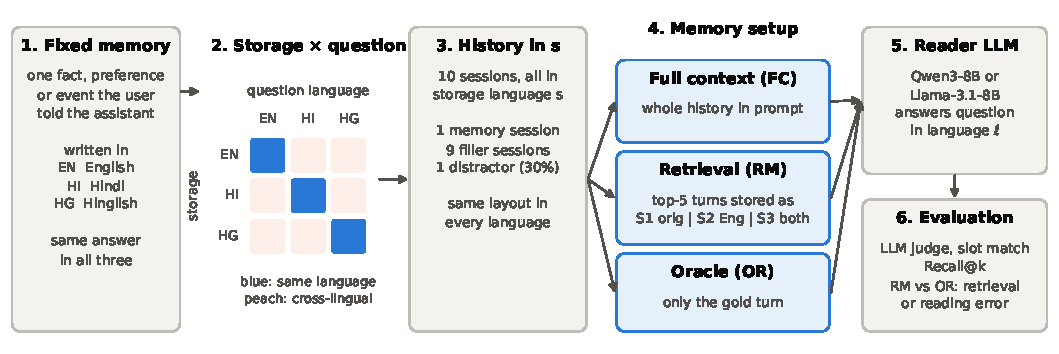
\includegraphics[width=\textwidth]{figures/fig0_method_overview.pdf}
\caption{Overview of the evaluation. A fixed memory is written in three languages, placed in a history in the storage language and queried in a question language. Comparing retrieval memory with the oracle separates retrieval errors from reading errors.}
\label{fig:method}
\end{figure*}

% ---------------------------------------------------------------------
\section{Related Work}
\label{sec:related}

\subsection{Long-term memory in LLM agents}
Research on long-term conversational memory began with multi-session dialogue, where retrieving or summarising earlier sessions outperformed a fixed context window~\citep{xu2022goldfish}.
Later systems treat memory as an explicit store that the agent writes, retrieves and updates~\citep{packer2023memgpt,zhong2024memorybank,chhikara2025mem0,xu2025amem}.
Benchmarks evaluate these systems on question answering over very long conversations~\citep{maharana2024locomo}, on five abilities that include temporal reasoning and knowledge updates~\citep{wu2025longmemeval}, and on incremental multi-turn input~\citep{hu2026memoryagentbench}.
LongMemEval also decomposes memory into indexing, retrieval and reading stages~\citep{wu2025longmemeval}.
This body of work shows that agents lose information over long horizons, but it measures that loss in English only.

Our work keeps the memory task of these benchmarks and derives its items from LongMemEval.
We add a controlled language dimension that none of them varies.
We also reuse the retrieval and reading decomposition, and we measure it separately for each pair of storage and query languages.

\subsection{Cross-lingual retrieval and question answering}
Cross-lingual question answering pairs a question in one language with a context in another.
MLQA introduced this setting over parallel Wikipedia paragraphs in seven languages, including Hindi~\citep{lewis2020mlqa}.
MLNeedle extended it to long contexts and found that models struggle when the relevant passage is in a non-English language~\citep{hengle2025mlneedle}.
In retrieval-augmented generation, models often answer in the wrong language~\citep{liu2025xrag}, and evaluation must tolerate different spellings of named entities~\citep{chirkova2024mrag}.
Studies of model internals suggest that multilingual models process meaning in a space close to English~\citep{wendler2024llamas}, and translating non-English input into English often improves accuracy~\citep{etxaniz2024selftranslate}.

These studies concern encyclopedic or news documents, and MLNeedle keeps every question in English.
We study personal memories that a user disclosed in conversation, and we vary the question language as well as the storage language.
Our English-translation condition tests the translation idea of \citet{etxaniz2024selftranslate} inside a memory store.
Concurrent work on cross-lingual web research reports drops even when the correct evidence is given~\citep{lu2026xbcp}, which matches the motivation for our oracle condition.

\subsection{Code-switching and multilingual agents}
Code-switching benchmarks such as GLUECoS and LinCE established Hindi--English mixing as a research topic~\citep{khanuja2020gluecos,aguilar2020lince}.
Recent studies show that LLM comprehension drops on code-switched input, and that the size of the drop depends on which language provides the grammatical frame~\citep{mohamed2026lostinthemix}.
Models also misjudge the language in which a code-switching user expects an answer~\citep{oh2026ola}.
For agents, tool-using models keep only part of their behaviour when the same task arrives in another language, because they route non-English tasks through English~\citep{mukherjee2026policyretention}.

None of these studies evaluates memory.
Two concurrent resources come closest.
A bilingual English--Vietnamese memory dataset mixes languages across events, but each question exists in one language only~\citep{nguyendang2026lhmemory}, and another study crosses storage and query languages for captioned photographs in a single commercial memory system~\citep{kim2026wontopos}.
Table~\ref{tab:related} positions our work against the closest studies.

\begin{table}[t]
\centering\small\setlength{\tabcolsep}{3pt}
\begin{tabular}{lccccccc}
\toprule
Work & Mem & St & Q & Mt & \HI & CM & Rep \\
\midrule
LongMemEval & \yes & \no & \no & \no & \no & \no & \partly \\
LoCoMo & \yes & \no & \no & \no & \no & \no & \partly \\
EN/VI memory set & \yes & \partly & \partly & \no & \no & \partly & \no \\
MLQA & \no & \yes & \yes & \yes & \yes & \no & \no \\
MLNeedle & \no & \yes & \no & \yes & \yes & \no & \no \\
XRAG & \no & \partly & \yes & \partly & \no & \no & \no \\
XBCP & \no & \yes & \no & \yes & \no & \no & \no \\
\textbf{Ours} & \yes & \yes & \yes & \yes & \yes & \yes & \yes \\
\bottomrule
\end{tabular}
\caption{Positioning against the closest work. Mem means personal or agent memory, St and Q mean the storage and query languages vary, Mt means the content is matched across languages, \HI\ means Hindi is included, CM means code-mixed text is included and Rep means memory representations are compared. The symbols \yes, \partly\ and \no\ mean yes, partly and no.}
\label{tab:related}
\end{table}

% ---------------------------------------------------------------------
\section{Methodology}
\label{sec:method}

\subsection{Task formulation}
An \emph{item} consists of a personal memory, a question about it and a gold answer.
The memory is a user turn that states a fact, a preference or an event.
The gold answer comes with accepted variants in all three scripts.
For a storage language $s$, we write the entire conversation history in $s$.
The question arrives in a new session in a query language $\ell$.
The nine pairs $(s,\ell)$ form a grid with three monolingual cells on its diagonal and six cross-lingual cells.

\subsection{Dataset construction}
We derive items from LongMemEval, which is released under the MIT licence~\citep{wu2025longmemeval}.
Its 64 single-session questions about user facts become \emph{fact} items.
Its 30 preference questions have open-ended answers, so we rewrite them as short-answer questions.
For example, a question about video-editing resources becomes ``Which video editing software do I enjoy using?'', with the answer Adobe Premiere Pro.
We build \emph{event} items from 87 user turns that contain an explicit calendar date.
We keep an item only if one user turn answers it, the answer is short, the answer is personal and the text translates naturally into Hindi.
The resulting pool holds 150 items, with 50 facts, 50 preferences and 50 events.
This paper reports a pilot with 30 of these items, ten of each type, and three unanswerable control questions.

Each item contains a memory turn, an assistant reply that never repeats the answer, a short follow-up exchange and two equivalent wordings of the question.
In 30\% of items we add a \emph{distractor}, which is a similar statement about another person with a different value, such as ``my sister's commute is only 20 minutes''.
Hindi verbs mark the gender of the speaker, so we fix the user's gender for each item and balance it within each memory type.
Hindi text uses Devanagari with brand names in Latin letters, and Hinglish uses Roman letters with Hindi grammar.
An LLM drafted all translations.
Automatic checks then confirm that the answer appears in the memory turn in every language and never appears in the replies or questions.
They also confirm that each distractor contains its own value and that verb gender matches the user.
An LLM review and a spot-check by the team followed, and they led to one correction.

\subsection{Conversation histories}
Each history contains ten sessions, which are the memory session and nine filler sessions taken from LongMemEval.
Qwen3-8B translated the filler sessions into Hindi and Hinglish.
A plain prompt produced Devanagari in 48\% of the Hinglish filler turns, so we added worked examples, a fallback that romanises the Hindi translation and a quality check that stops the run.
We write the filler in the storage language, so a Hindi memory never stands out against English text.
A fixed random seed per item chooses the filler sessions, the position of the memory and the position of the distractor, and these choices are identical in all three languages.

\subsection{Memory setups and representations}
We compare three ways of giving the model access to its memory.
In the \emph{full context} setup (FC), the whole history is part of the prompt.
In the \emph{retrieval memory} setup (RM), we index every user turn and show the model the five turns most similar to the question, ranked by the BGE-M3 embedding model~\citep{chen2024bgem3}.
RM uses one of three representations.
S1 stores the original text, S2 stores an English translation of each memory and translates the question as well, and S3 stores both versions.
In the \emph{oracle} setup (OR), the model receives only the correct turn and the distractor, if the item has one.
The oracle removes retrieval, so the difference between RM and OR measures retrieval errors, and the errors that remain under OR are reading errors.

% ---------------------------------------------------------------------
\section{Experimental Setup}
\label{sec:setup}

\paragraph{Input and output.}
Table~\ref{tab:io} shows one instance from the pilot.
The input consists of a fixed English instruction, the history or the retrieved memories, and the question.
The expected output is one short sentence that contains the gold answer, in any language or script.
Appendix~\ref{app:prompts} lists all prompts.

\begin{table}[t]
\centering\small
\begin{tabularx}{\columnwidth}{@{}lX@{}}
\toprule
\textbf{Storage (\HI)} & \hi{मैं आजकल रोज़ ऑफिस आते-जाते ऑडियोबुक्स सुनती हूँ, एक तरफ़ का सफ़र 45 मिनट का होता है।} The history also contains nine Hindi filler sessions and the distractor \hi{मेरी बहन का ऑफिस तो बस एक तरफ़ 20 मिनट दूर है।} \\
\textbf{Question (\HG)} & \emph{Mera office jaane mein ek side kitna time lagta hai?} \\
\textbf{Gold} & 45 minutes each way. The distractor value is 20 minutes. \\
\textbf{Llama} & \hi{मुझे आपकी पिछली बातचीत की याद है, जहां आपने बताया था कि आपकी बहन का ऑफिस तो बस एक तरफ़ 20 मिनट दूर है।} The answer is incorrect, takes the distractor value and is in Hindi. \\
\textbf{Qwen} & \hi{एक तरफ़ का सफ़र 45 मिनट का होता है।} The answer to the second wording is correct. \\
\bottomrule
\end{tabularx}
\caption{Real model outputs for item F001 with the memory stored in Hindi, the question asked in Hinglish and the full history in the prompt.}
\label{tab:io}
\end{table}

\paragraph{Models.}
The readers are Qwen3-8B~\citep{yang2025qwen3} with its reasoning mode disabled and Llama-3.1-8B-Instruct~\citep{grattafiori2024llama3}.
Both models officially support Hindi.
We use greedy decoding at 16-bit precision with vLLM~\citep{kwon2023vllm} on two NVIDIA T4 GPUs from the free Kaggle tier.
The pilot produces 4,158 answers per reader, which are 33 items in 9 cells with 7 setups and 2 wordings, and the full run takes about 1.5 hours.

\paragraph{Baselines.}
The monolingual diagonal is the reference for each cross-lingual cell.
Storage of the original text (S1) is the baseline for the English and dual representations.
BM25~\citep{robertson2009bm25}, a keyword-matching retriever, serves as a lexical baseline next to the embedding retrievers BGE-M3 and multilingual-E5~\citep{wang2024me5}.
The full-context setup is the baseline without a memory module, and the oracle is an upper bound for reading.

\paragraph{Metrics.}
\emph{Accuracy} is the share of answers that an LLM judge labels correct.
\emph{Recall@k} is the share of questions for which the correct memory turn appears among the top $k$ retrieved turns.
\emph{Reading error} is the share of wrong answers among questions where retrieval succeeded.
We also count \emph{distractor errors}, \emph{false abstentions}, which are ``I don't know'' answers to answerable questions, and \emph{invented answers} to the unanswerable controls.
The \emph{noise floor} is the rate at which the two equivalent wordings of a question receive different scores.
We pair all comparisons by item, report 95\% bootstrap confidence intervals and use exact sign tests~\citep{mcnemar1947} with Holm correction for multiple tests~\citep{holm1979}.

\paragraph{Evaluation protocol.}
Automated evaluation covers answer matching against the accepted variants, retrieval ranks and the detection of the answer's script.
An LLM judge~\citep{zheng2023judging}, Qwen3-14B, labels every answer as correct, incorrect or no answer.
To test the judge, an independent LLM annotator (Claude) labelled a stratified sample of 200 answers.
The two agree on 96.5\% of labels, with Cohen's $\kappa=0.85$, a chance-corrected agreement score where 1 means perfect agreement.
Human evaluation in this pilot is limited to an informal spot-check by the team, and the main study adds two human annotators.
Our ablations vary the memory setup, the representation, the retriever and the wording of the question.

% ---------------------------------------------------------------------
\section{Results}
\label{sec:results}

\begin{figure*}[t]
\centering
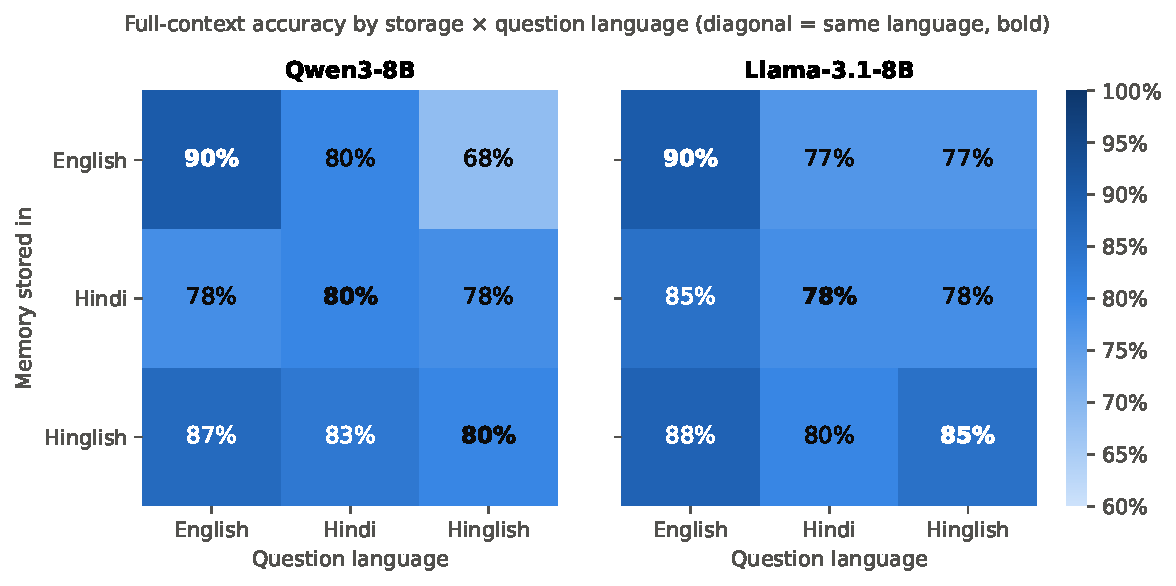
\includegraphics[width=0.82\textwidth]{figures/fig1_fc_accuracy_heatmap.pdf}
\caption{Full-context accuracy for each pair of storage and question language. Each cell covers 30 items with two wordings each. Bold cells are monolingual.}
\label{fig:heatmap}
\end{figure*}

\subsection{RQ1. Does accuracy drop across languages?}
Table~\ref{tab:gap} compares monolingual and cross-lingual accuracy for each setup, and Figure~\ref{fig:heatmap} shows the full-context grid.
The main takeaway is that the pilot shows no reliable overall gap.
In full context, cross-lingual accuracy is about four points lower for both models, but both confidence intervals include zero.
The two equivalent wordings of a question disagree on 18\% to 24\% of items in this setup, so a four-point difference lies within the noise of a 30-item pilot.

A secondary takeaway is that the retrieval and oracle setups are close to their ceiling.
BGE-M3 places the correct memory among the top five turns in 97\% to 100\% of questions in every cell, so retrieval rarely fails.
This ceiling triggers our pre-registered rule to make the main study harder.
The weakest single cell in Figure~\ref{fig:heatmap} is Qwen with English storage and a Hinglish question, at 68\%.

\begin{table}[t]
\centering\small\setlength{\tabcolsep}{4pt}
\begin{tabular}{llccc}
\toprule
Reader & Setup & Mono & Cross & Gap [95\% CI] \\
\midrule
\multirow{4}{*}{Qwen3} & FC & 83.3 & 79.2 & 4.2 [$-$0.6, 9.2] \\
 & RM-S1 & 91.1 & 89.4 & 1.7 [$-$0.8, 4.4] \\
 & RM-S2 & 92.2 & 88.3 & 3.9 [0.6, 7.8] \\
 & OR-S1 & 95.0 & 95.6 & $-$0.6 [$-$3.6, 2.5] \\
\midrule
\multirow{4}{*}{Llama} & FC & 84.4 & 80.8 & 3.6 [$-$1.1, 8.6] \\
 & RM-S1 & 94.4 & 94.7 & $-$0.3 [$-$3.9, 3.3] \\
 & RM-S2 & 96.7 & 96.7 & 0.0 [$-$2.2, 2.2] \\
 & OR-S1 & 97.8 & 96.9 & 0.8 [$-$1.7, 3.3] \\
\bottomrule
\end{tabular}
\caption{Accuracy in percent on monolingual and cross-lingual cells, paired by item. Appendix~\ref{app:extra} reports the remaining setups.}
\label{tab:gap}
\end{table}

\subsection{RQ2. Is one direction easier?}
We compare each cross-lingual cell in Figure~\ref{fig:heatmap} with its mirror image.
The main takeaway is a possible asymmetry for Qwen in full context.
A memory stored in Hinglish and asked about in English is answered correctly more often than the reverse, on 11 items against 2 items, with a difference of 18 points and a 95\% interval from 7 to 32 points.
The exact test gives $p=0.022$, but we ran 42 such tests, and the effect is not significant after Holm correction.

The secondary takeaway is that Llama points in the same direction, on 8 items against 3.
This pattern fits the view that models route non-English input through English~\citep{wendler2024llamas,mukherjee2026policyretention}.
We treat it as a hypothesis for the main study.

\subsection{RQ3. Does code-switching add errors?}
Table~\ref{tab:qvs} splits full-context accuracy by one language at a time.
The main takeaway is that the question language matters more than the storage language.
English questions score highest for both models, while Hindi and Hinglish questions score lower, with the lowest result for Hinglish questions to Qwen.
Code-switching therefore hurts mainly when it appears in the question.
This agrees with reports that code-switched input reduces comprehension~\citep{mohamed2026lostinthemix}.

The secondary takeaway is that storage in Hinglish does not hurt.
Accuracy varies little across storage languages, and Hinglish storage scores slightly higher than English or Hindi storage for both models.
Appendix~\ref{app:extra} shows the same comparison as a figure.

\begin{table}[t]
\centering\small\setlength{\tabcolsep}{5pt}
\begin{tabular}{lcccccc}
\toprule
 & \multicolumn{3}{c}{By question language} & \multicolumn{3}{c}{By storage language} \\
\cmidrule(lr){2-4}\cmidrule(lr){5-7}
Reader & \EN & \HI & \HG & \EN & \HI & \HG \\
\midrule
Qwen3 & 85.0 & 81.1 & 75.6 & 79.4 & 78.9 & 83.3 \\
Llama & 87.8 & 78.3 & 80.0 & 81.1 & 80.6 & 84.4 \\
\bottomrule
\end{tabular}
\caption{Full-context accuracy in percent, averaged over the other language.}
\label{tab:qvs}
\end{table}

\begin{figure*}[t]
\centering
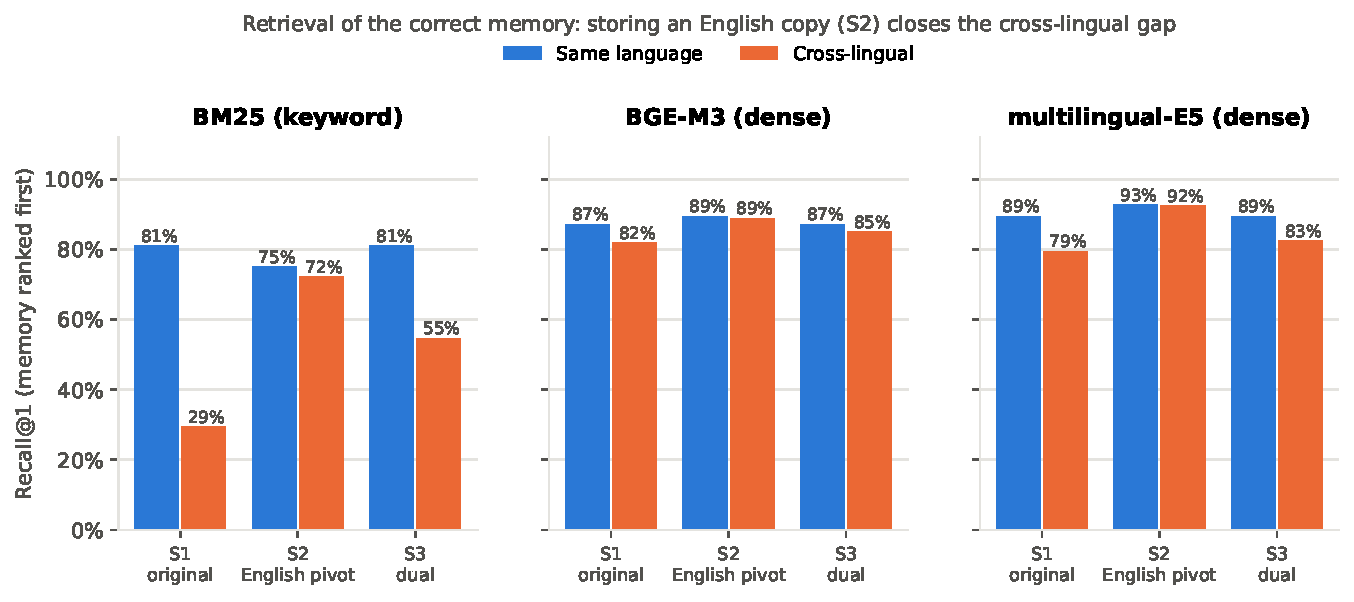
\includegraphics[width=0.9\textwidth]{figures/fig2_retrieval_recall_at_1.pdf}
\caption{Recall@1 of the correct memory for each retriever and representation, on monolingual and cross-lingual cells.}
\label{fig:retrieval}
\end{figure*}

\subsection{RQ4. Which representation preserves memory?}
Figure~\ref{fig:retrieval} shows how often each retriever ranks the correct memory first.
The main takeaway is that an English copy rescues keyword retrieval across scripts.
With the original text, BM25 ranks the correct memory first in 81\% of monolingual questions but in only 29\% of cross-lingual ones, because English and Devanagari share no words.
Storing an English copy raises the cross-lingual rate to 72\%, and storing both versions reaches 55\%.

The secondary takeaway concerns embedding retrievers.
They find the memory among the top five in almost every case, but they still rank it first less often across languages, with BGE-M3 falling from 87\% to 82\% and multilingual-E5 from 89\% to 79\%.
The English copy removes this loss for both retrievers.
Retrieval is rarely the bottleneck in the pilot, since Qwen misses the memory in 0.8\% of cross-lingual S1 questions but answers 9.8\% of the retrieved cases wrongly.

\subsection{Error analysis}
Most full-context errors are false abstentions.
Of 105 errors by Qwen and 97 errors by Llama, 69 and 71 respectively are ``I don't know'' answers, so the models fail to find the memory more often than they misremember it.
Distractor errors are rare, and Table~\ref{tab:io} shows one in which Llama reports the sister's commute instead of the user's.
Events with explicit dates are the easiest memory type, and preferences are the hardest.

On the unanswerable controls, Qwen gives a specific answer in 18.5\% of cases and Llama in 7.9\%.
For example, Llama invents an app called ``Focus@will'' when asked which audiobook app the user uses.
Qwen answers English questions in English in 96\% of cases, while Llama answers them in Hindi or Hinglish in 45\% of cases.
Both models answer a quarter or more of Hinglish questions in Devanagari script.
This matches the language confusion reported for code-switched prompts~\citep{oh2026ola}.
Translation can also distort content, as in a Hindi answer that renders ``short-grain rice'' as \hi{छोटा गेहूँ चावल}, which means ``short wheat rice''.

Storage in Hindi is also more expensive.
The same history needs 4.1 times as many tokens in Hindi as in English for the Qwen tokenizer and 2.3 times as many for the Llama tokenizer, as Appendix~\ref{app:extra} shows.
A Hindi history is therefore longer for the model, which the main study must report as a property of the language.

\subsection{Lessons and next steps}
\label{sec:next}
The pilot validated the pipeline and exposed three problems that we fixed, namely Devanagari in Hinglish filler, a token-counting bug and a disk limit on Kaggle (Appendix~\ref{app:dev}).
The main study will use all 150 items, which gives 80\% power for paired gaps of about 12 points.
It will make retrieval harder with about 20 sessions per history and distractors in half of the items, because 30 Hindi sessions would exceed the context length of Qwen3-8B.
It will also add a human evaluation with two annotators and ablations on longer histories, indirect questions, Devanagari digits and English-framed Hinglish.

% ---------------------------------------------------------------------
\section{Conclusion}
We presented a controlled evaluation of cross-lingual agent memory that holds each personal memory fixed while varying its storage and query language across English, Hindi and Hinglish.
A 30-item pilot shows that an English representation of each memory protects retrieval across scripts.
It also shows that the language of the question matters more than the language of storage, and that most failures are false abstentions.
The overall cross-lingual gap is small compared with the measurement noise at pilot scale, and our 150-item study is designed to measure it.

% ---------------------------------------------------------------------
\section*{Limitations}
This study is a pilot, and its 30 items give limited statistical power.
An LLM drafted and reviewed the Hindi and Hinglish items, and the team only spot-checked them.
Machine translation produced the filler sessions, which contain minor errors, although the evaluation never scores them.
We validated the LLM judge against a second LLM and not against human annotators.
The judge also accepted two invented answers to unanswerable questions, so the reported rates of invented answers may be too low.
The source data from LongMemEval reflects mostly American contexts.
We tested two open models with eight billion parameters only, and retrieval was near its ceiling, so the pilot cannot yet show how retrieval errors propagate to answers.

\section*{Acknowledgements}
We thank Kaggle for free GPU access and the authors of LongMemEval for releasing their data.

\noindent\textbf{AI Use Statement.}
As the course permits, we used Claude (Anthropic) throughout the project.
It searched and verified literature, helped design the experiment, drafted the dataset items and their translations, wrote the evaluation pipeline, ran the analysis, produced the figures, labelled answers as an LLM annotator and drafted this paper.
The authors directed the work, reviewed the outputs and take responsibility for all content.

\bibliography{custom}

% ---------------------------------------------------------------------
\appendix

\section{Prompt Templates}
\label{app:prompts}
\small
\paragraph{Reader instruction.}
\emph{You are a personal assistant with memory of your past conversations with this user. Answer the user's question using only what the user told you in past conversations. Answer in one short sentence, in the same language as the question. If the information is not in the past conversations, say that you don't know.}

\paragraph{Reader input.}
In the full-context setup, the input lists every session as ``[Session 1] User \ldots\ Assistant \ldots'' and ends with ``Current question \{q\}''.
In the retrieval and oracle setups, the input lists the memories under the heading ``Relevant memories from past conversations (may be incomplete or irrelevant)'' and ends with the question.
Under S3, each memory appears as ``\{original\} (English \{translation\})''.

\paragraph{Judge.}
The judge receives the question, the gold answer with its accepted variants and the model answer.
It replies with one word, CORRECT if the answer states the gold information without contradiction, INCORRECT if it is wrong, incomplete or lists several candidates, and NO\_ANSWER if it says it does not know.
For unanswerable controls, the labels are ANSWERED and NO\_ANSWER.

\paragraph{Translator.}
\emph{Translate the following text to English. It may be Hindi, Hinglish (romanized Hindi) or English. Keep names, numbers and dates exactly. Output only the translation.}
\normalsize

\section{Additional Results}
\label{app:extra}

\begin{table}[h]
\centering\small\setlength{\tabcolsep}{4pt}
\begin{tabular}{llccc}
\toprule
Reader & Setup & Mono & Cross & Gap [95\% CI] \\
\midrule
\multirow{3}{*}{Qwen3} & RM-S3 & 92.2 & 91.4 & 0.8 [$-$1.9, 3.6] \\
 & OR-S2 & 97.2 & 95.6 & 1.7 [0.3, 3.3] \\
 & OR-S3 & 97.8 & 96.9 & 0.8 [$-$1.4, 3.1] \\
\midrule
\multirow{3}{*}{Llama} & RM-S3 & 96.7 & 95.6 & 1.1 [$-$2.5, 4.4] \\
 & OR-S2 & 97.8 & 98.3 & $-$0.6 [$-$2.2, 0.8] \\
 & OR-S3 & 97.2 & 97.2 & 0.0 [$-$2.8, 2.5] \\
\bottomrule
\end{tabular}
\caption{Remaining setups of Table~\ref{tab:gap}.}
\label{tab:gap_extra}
\end{table}

Table~\ref{tab:gap_extra} completes Table~\ref{tab:gap}.
Figure~\ref{fig:qvs} shows the comparison of Table~\ref{tab:qvs} as bars, and Figure~\ref{fig:tokens} shows the token cost of each storage language.

\begin{figure}[h]
\centering
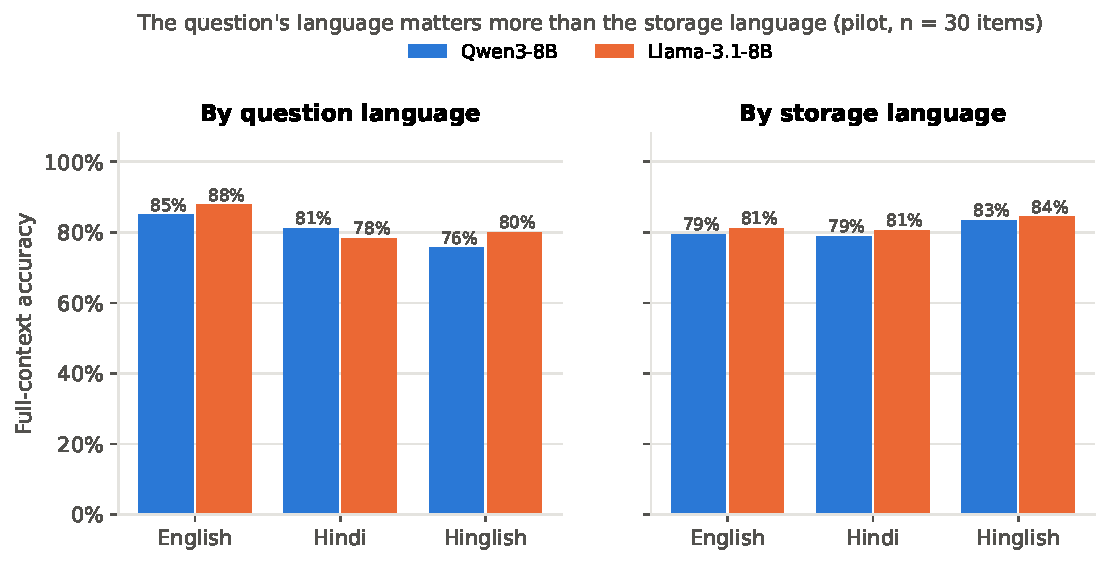
\includegraphics[width=\columnwidth]{figures/fig4_query_vs_storage_language.pdf}
\caption{Full-context accuracy by question language and by storage language.}
\label{fig:qvs}
\end{figure}

\begin{figure}[h]
\centering
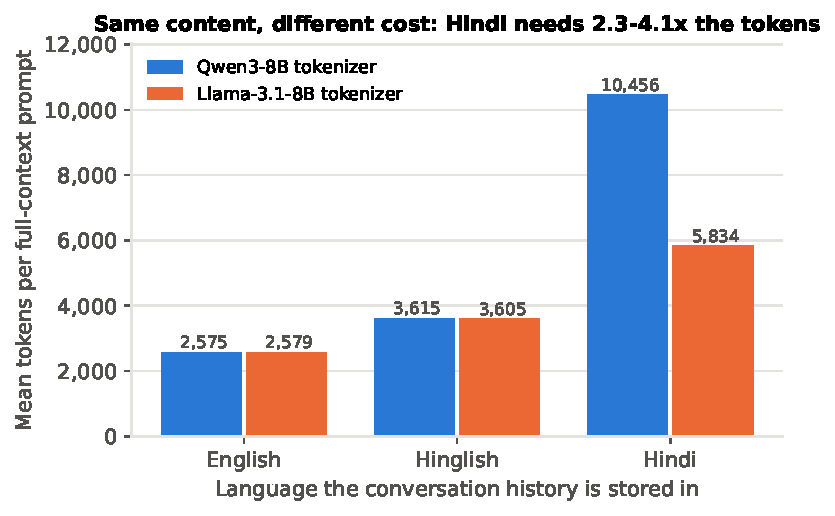
\includegraphics[width=0.9\columnwidth]{figures/fig3_token_cost.pdf}
\caption{Mean number of tokens per full-context prompt by storage language.}
\label{fig:tokens}
\end{figure}

\section{Changes Made During the Pilot}
\label{app:dev}
We ran all seven setups in the pilot, although the plan required three, because the extra setups cost little compute.
The pilot used draft translations because of the course deadline.
A plain prompt wrote 77 of 160 Hinglish filler turns in Devanagari, so we added worked examples, a romanising fallback and a check that stops the run if more than 5\% of turns fail.
The token check first counted dictionary keys under transformers 5, which always gave 2, and we fixed it.
The measured token ratios show that 30 Hindi sessions would exceed the 32k context of Qwen3-8B, so the long-history ablation will use about 20 sessions.
Finally, we test direction effects per item and correct over all 42 tests.

\end{document}
